% !TeX spellcheck = en_US
\section{Problem 9}

In figure~\ref{fig:prob9_given_contour_plot}, we are given a contour plot and we are asked to draw one gradient step for the three following algorithms:
\begin{itemize}
	\item Gradient Descent,
	\item Natural Gradient (\textit{Newton's method}) and
	\item Adagrad or RMSprop.
\end{itemize}

\begin{figure}[htpb]
	\centering
	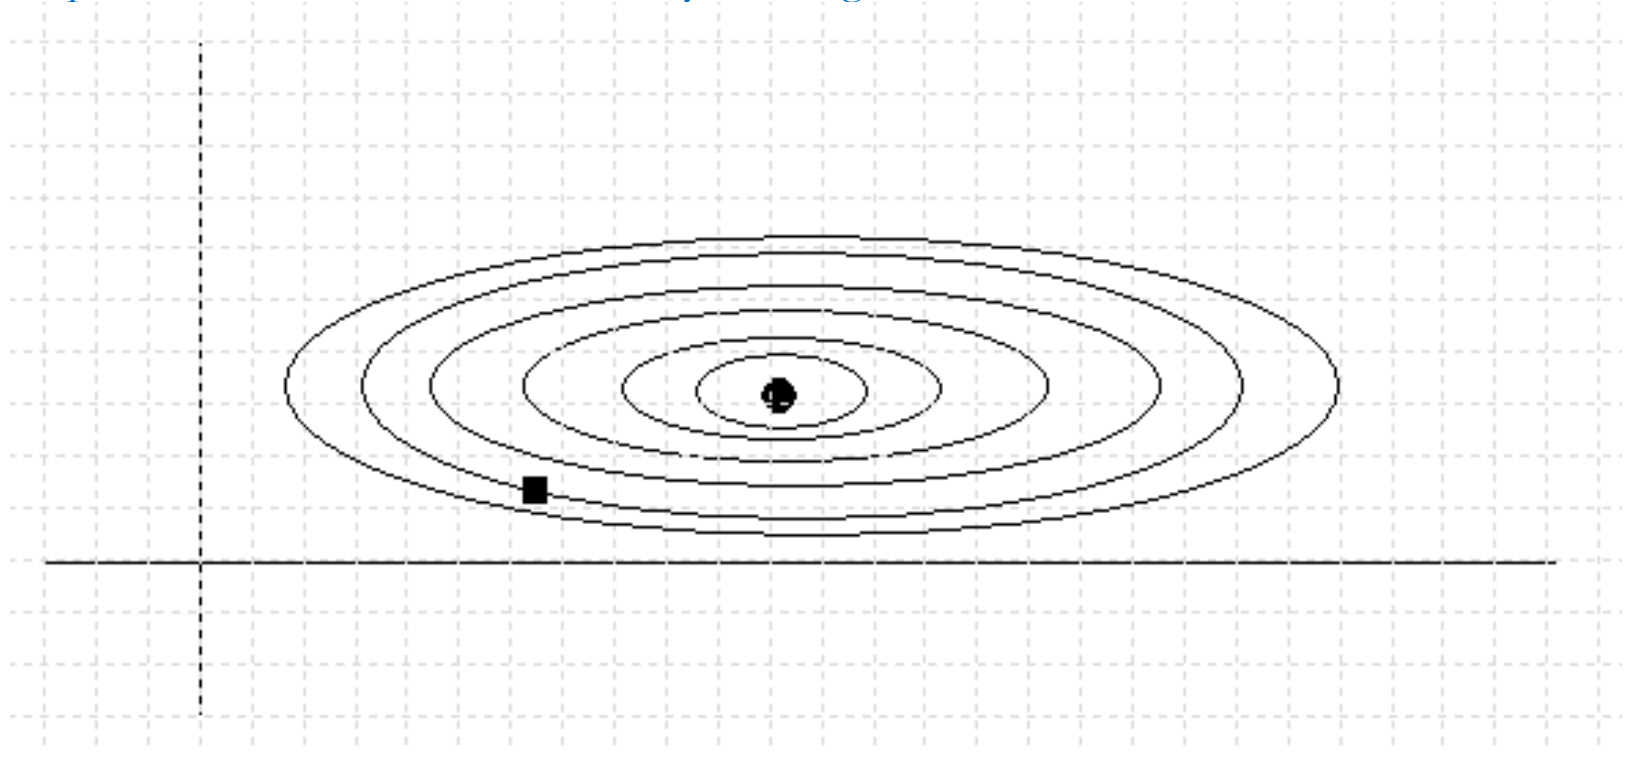
\includegraphics[width=0.7\textwidth]{../Problem 9/contour_plot.png}
	\caption{Given contour plot.}
	\label{fig:prob9_given_contour_plot}
\end{figure}

\subsection{Gradient Descent}

Gradient Descent calculates the next step as follows. First, the gradient is calculated using a \textit{mathematical expression}. Then, it progresses through the contour plot in the opposite direction of gradient.

This is done repeatedly, until a local minimum is found and converges there.\\

In this problem, we don't have any mathematical expression in order to calculate the gradient, so we will approximate it \underline{visually} from the contour plot.

Looking at the starting point in figure~\ref{fig:prob9_given_contour_plot} (\textit{the rectangle}), 
the gradient at this point is perpendicular to the contour line and points in the direction of the steepest increase in function value.\\
Following the algorithm, gradient descent moves in the \textit{opposite direction of the gradient}, which is the direction of the steepest decrease in function value.

Gradient and direction of movement are shown in figure~\ref{fig:prob9_contour_gd}.

\begin{figure}[htpb]
	\centering
	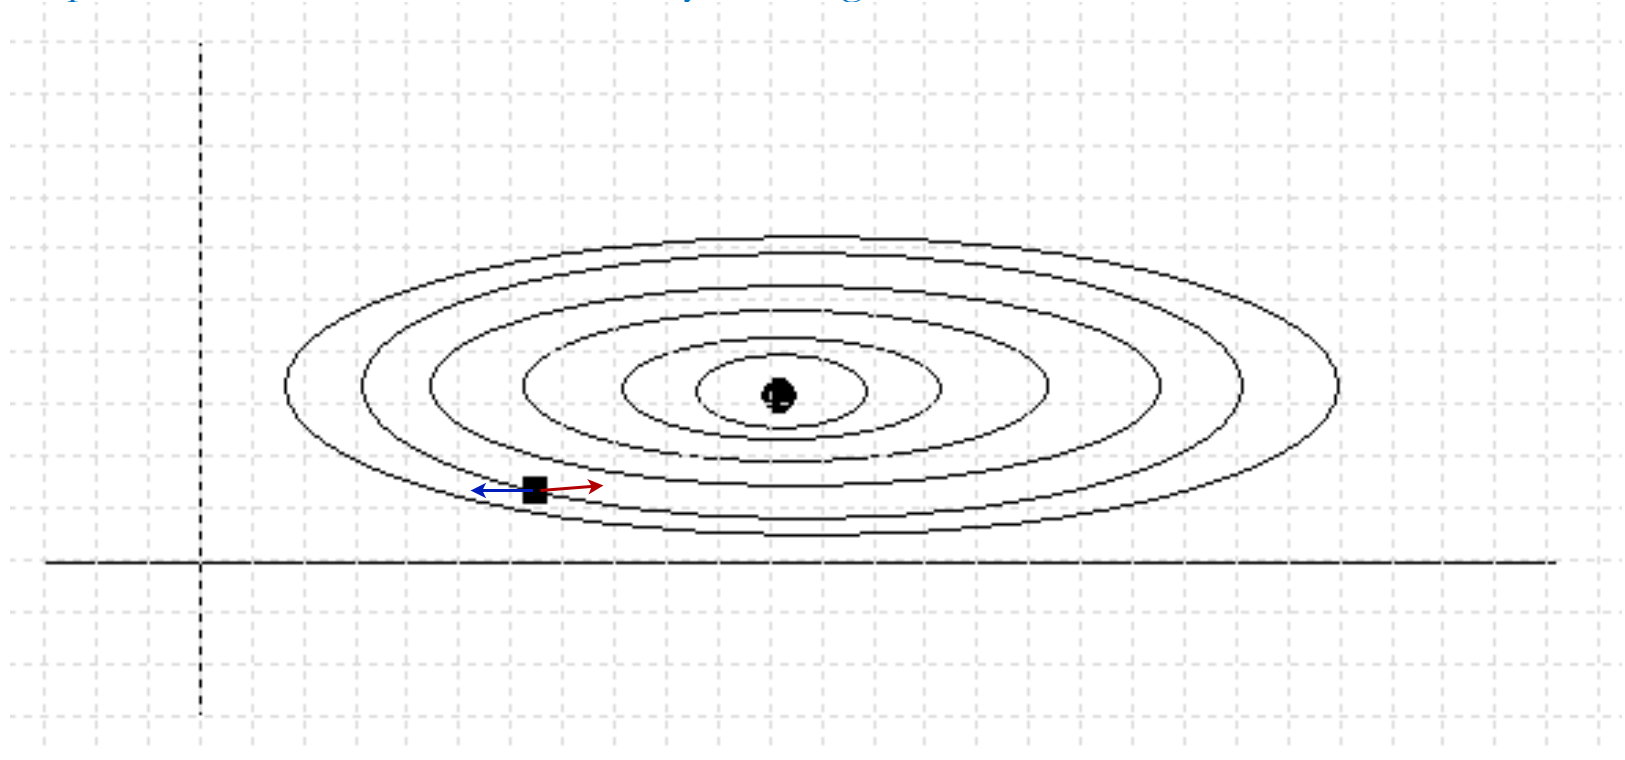
\includegraphics[width=0.7\textwidth]{../Problem 9/contour_gd.png}
	\caption{First step of gradient descent. Blue arrow represents the \textbf{gradient} on the first step and red arrow represents the \textbf{step} of the algorithm.}
	\label{fig:prob9_contour_gd}
\end{figure}
